%%%%(c)
%%%%(c)  This file is a portion of the source for the textbook
%%%%(c)
%%%%(c)    Abstract Algebra: Theory and Applications
%%%%(c)    Copyright 1997 by Thomas W. Judson
%%%%(c)
%%%%(c)  See the file COPYING.txt for copying conditions
%%%%(c)
%%%%(c)
\chap{Further topics in Cryptography}{Crypto}
\section{Diffie Hellman Key Exchange}\label{sec:DHKE:1}

In order to share a private message over a public domain a sender must  "lock" or encrypt their message using a \emph{key}\index{key! in cryptogaphy}.  In cryptography a  key is a special piece of information (usually a number)  that is required to encrypted and decrypt data that is shared between the sender and receiver.  The Diffie Hellman Key Exchange (DHKE) focuses on three types of keys: public, private and symmetric.  A \emph{Public Key}\index{Public Key! in cryptography} can be widely distributed, and is used for encrypting messages.  A\emph{Private Key}\index{Private Key! in cryptography} is only known to the sender, and is used for decrypting messages.  Finally, a \emph{Symmetric Key}\index{Symmetric Key! in cryptography} is known by the sender and receiver, and is used to encypt and decrypt messages.  The security that a key exchange offers is so profound that it is embedded into almost every technology we use today.  Some examples of key exchange can be seen in media applications, cellular phones, banking, and emails. 

So, how do you establish a key?  Looking at this problem from the most fundamental level you would simply tell the other parties what the private key is, but this method is inefficient and is susceptible to eavesdroppers.  So, how do you establish a key over an unsecure network without compromising your data to potential eavesdroppers?  The Diffie-Hellman Key Exchange (DHKE) is one possible solution.  The DHKE is a public key algorithm that is used to establish a key between two parties over an unsecure network.  Note that the DHKE is not used for encryption/decryption of messages, but only to establish a key that can be used to encrypt/decrypt subsequent messages.  

The steps in the DHKE algorithm are as follows (see also Figure~\ref{fig:DH:DHKE_1}):
 \begin{enumerate}[Step 1.]
 \item Prior to sending data, Moses and Rachael agree upon a prime number $p$ and a base number $g$ where $g$ is a primitive root of $p$; 
\item Moses chooses a secret integer $n$, and sends Rachael $ \bmod (g^n , p)$;
\item Rachael chooses a secret integer $m$, and sends Moses  $ \bmod (g^m , p)$;
\item Moses computes $ \bmod ( \bmod (g^m , p)^n , p ) = K_1$;
\item Rachael computes $ \bmod (\bmod (g^n , p)^m , p ) = K_2$;
\end{enumerate} 
\begin{figure}[htb]
	   \center{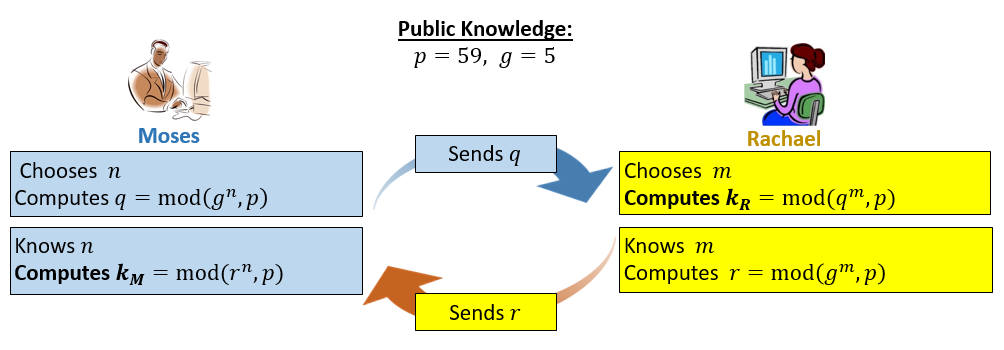
\includegraphics[width=5in]
	         {images/DHKE_1.png}}
	  \caption{\label{fig:DH:DHKE_1} Key exchange between Moses and Rachael }
\end{figure}
It turns out that when $K_1$ and $K_2$ are computed by the above procedure, then $K_1$ is always equal to $K_2$.  You will show this in the following exercise.

\begin{exer}\\
Fill in the blanks in the following proof that  $K_1$ is always equal to  $K_2$.\\
  	\begin{proof} 
		\begin{align*} 
		K_1 &=   \bmod ( \bmod (g^m , p)^n , p ) 
           	\\&=  \bmod ( \bmod ((g^m)^{\underline{~~~~}} , p) , p )&& \text{(modular arithmetic)}	%ans: \bmod ( \bmod ((g^m)^n , p) , p )&& \text{(modular arithmetic)}
		\\&= \bmod ( \bmod ((g^{mn}) , p) , p )&&  \text{(rules of exponents)}	%ans: \bmod ( \bmod ((g^{mn}) , p) , p )&&  \text{(rules of exponents)}	
           	\\&= \bmod ( \bmod (\underline{~~~~~~}) , p) , p ) &&\text{(rules of exponents)}	%ans: \bmod ( \bmod ((g^{nm}) , p) , p ) &&\text{(rules of exponents)}
           	\\&= \bmod ( \bmod ((\underline{~~~~~~})^m , p) , p )  &&\text{(rules of exponents)}	%ans:  \bmod ( \bmod ((g^n)^m , p) , p )  &&\text{(rules of exponents)}
           	\\&= \bmod ( \bmod ((\underline{~~~~~~} , \underline{~~~~~~})^m , p )&&\text{(modular arithmetic)}   	%ans: \bmod ( \bmod ((g^n , p)^m , p )&&\text{(modular arithmetic)}
		\\&= K_2
		\end{align*} 
   	Thus, $K_1 = K_2 = K$ is the symmetric private key.\\

  	\end{proof}
\end{exer}

In order to make things clearer, we give a simple example to show how key exchange works (note that this example is much too simple to be used in practice, but it does at least show the procedure):

 \begin{eg} Key Exchange between a sender and receiver (Moses and Rachael) using the DHKE is shown in the following steps.
\begin{enumerate}[Step 1.]
\item Prior to sending data, Moses and Rachael agree $p$ = 13 and $g$= 7; 
\item Moses chooses $n$ = 2, and sends Rachael $\bmod (7^2 , 13) = 10$;
\item Rachael chooses $m$ = 8, and sends Moses $\bmod (7^8  , 13) = 3 $;
\item Moses computes $\bmod ((3)^2 , 13 ) = 9$;
\item Rachael computes $\bmod ((10)^8 , 13 ) = 9$;
\item Moses and Rachael share the number 9;
\end{enumerate}
\end{eg}
It is important to choose a large prime number $p$, in order to decrease the chances of an eavesdropper cracking your code.  For example, internet protocols usually use a minimum of a 1024-bit prime number for $p$.  There are $2^{1023}$ different possibilities for 1024 bits (where the highest bit is a `1`), but how can you guarantee that the number is prime?

  \emph{Fermat's Little Theorem}\index{Fermat's Little Theorem! in cryptography} states that if $p$ is a prime number such that $p \nmid a$, and $a$ is an integer, then $1 \equiv \bmod(a^{p-1}, p)$.

\begin{eg} Let $p = 5$ and $a = 1, 2, 3, 4 \text{ and } 5$
$$ 5 \nmid 1 \implies \bmod(1^{5-1}, 5) \equiv 1$$
$$ \bmod(1^{4}, 5) \equiv 1$$
$$ \bmod(1, 5) \equiv 1$$
$$ 5 \nmid 2 \implies \bmod(2^{5-1}, 5) \equiv 1$$
$$ \bmod(2^{4}, 5) \equiv 1$$
$$ \bmod(16, 5) \equiv 1$$
$$ 5 \nmid 3 \implies \bmod(3^{5-1}, 5) \equiv 1$$
$$ \bmod(3^{4}, 5) \equiv 1$$
$$ \bmod(18	, 5) \equiv 1$$
$$ 5 \nmid 4 \implies \bmod(4^{5-1}, 5) \equiv 1$$
$$ \bmod(4^{4}, 5) \equiv 1$$
$$ \bmod(256, 5) \equiv 1$$
$$ 5 | 5 \text { (so the theorem does not apply)}$$
$$ \bmod(5^{5-1}, 5) \equiv 0$$
\end{eg}
Since all values of $a$ such that $1 \leq a \leq p$ are congruent to $1$, then Fermat's Little Theorem tells us that $p$ is prime, but are there numbers that exist that pass Fermat's Little Theorem but are not prime?  The answer is yes, these numbers are called \emph{Lucas-Carmichael Numbers}\index{Lucas-Carmichael Numbers! in cryptogaphy}.  (or \emph{pseudoprimes}\index{Pseudoprimes}) 

Performing exponentiation over a modulus is called \emph{discrete exponentiation}\index{discrete exponentiation! in cryptogaphy} and can quickly become incalculable, however you can overcome this by creating a repeated squaring formula using an excel spreadsheet.  See \emph{Chapter 7.2.3 RSA Exercises, Exercise 36} for instructions on how to create a spreadsheet to compute the following exercises.
 
\begin{exer}
Given $p$ = 32452867; $g$ = 54321; and $n$ = 876.  
\begin{enumerate}[(a)]
\item What number do you send?  
%ans: mod((54321)876, 32,452,867) = 19,439,625

\item You are then sent 31975948, what is the key? 
%ans: K = mod((31,975,948)876, 32,452,867) = 16,045,878

\item If $m$ = 123 what number does the other party calculate?
%ans: K = mod((19,439,625)123, 32,452,867) = 16,045,878
\end{enumerate}
\end{exer}\begin{exer}
Given $p$ = 86028157; $g$ = 98765; and $n$ = 123.  
\begin{enumerate}[(a)]
\item	What number do you send?  
%ans: mod((98765)123, 86,028,157) = 7,262,961

\item You are then sent 53161396, what is the key? 
%ans: K = mod((53,161,396)123, 86,028,157) = 35,164,864

\item If $m$ = 87 what number does the other party calculate?
%ans: K = mod((7,262,961)87, 86,028,157) = 35,164,864
\end{enumerate}
\end{exer}
The security of the DHKE leverages the easy computations of exponentials versus the difficulty of computing logarithms. 
Recall that the logarithm is the inverse operation of exponentiation.  For example, suppose $a = g^m$ , then the Discrete Logarithm (DL) of $a$ = $m$ and is expressed as    $\log_g a = m$.   

\begin{defn} \label{def:DLP}(\emph{Discrete Logarithm Problem})~~
The \emph{discrete logarithm problem}\index{discrete logarithm problem! in cryptogaphy} refers to the difficulty of finding logarithms modulo some integer. This is sometimes reffered to in cryptography as a \emph{one-way function}; easy to calculate but hard to invert. Let's look at an example, $\bmod(2^{4},  11) = 5$ is easy to solve, but $\bmod(2^{m},  11) = 5$ is more difficult to solve without computing the results. 
$$ \bmod(2^{1}, 11)=2$$
$$ \bmod(2^{2}, 11)=4$$
$$ \bmod(2^{3}, 11)=8$$
$$ \bmod(2^{4}, 11)=5$$
$$ \bmod(2^{5}, 11)=10$$
$$ \bmod(2^{6}, 11)=9$$
$$ \bmod(2^{7}, 11)=7$$
$$ \bmod(2^{8}, 11)=3$$
$$ \bmod(2^{9}, 11)=6$$
$$ \bmod(2^{10}, 11)=1$$

As you can see the results "jump" around, but each solution is equally likely to be any integer between 0 and 11.  This is the strength of the discrete logarithm problem, and the larger the modulus is the harder it is to solve.
\end{defn}
\begin{exer}
Use the Repeated Square spreadsheet from the previous Exercise to solve the following Discrete Logarithm Problems.  
\begin{enumerate}[(a)]
\item Given $ \bmod(7^{m}, 41)=28$, solve for $m$.
%ans: 29

\item Given $ \bmod(5^{m}, 73)=13$, solve for $m$.
%ans: 59

\item Given $ \bmod(17^{m}, 211)=161$, solve for $m$.
%ans: 161
\end{enumerate}
\end{exer}
Now that we have established that with a large enough modulus the DHKE is infeasable to crack; is there any way to successfully eavesdrop on Moses and Rachael's conversation without actually cracking the code?  Both Moses and Rachael seem confident with the security that the DHKE provides, since an Attacker would only be privy to $\mod (g^n , p)$ and $\mod (g^m , p)$ each of which cannot be used to decrypt the message since an Attacker would have to solve the discrete logarithm problem.

\begin{eg} Key Exchange between a sender and receiver (Moses and Rachael) using the DHKE is shown in the following steps.
\begin{enumerate}[Step 1.]
\item Prior to sending data, Moses and Rachael agree $p$ = 13 and $g$= 7; 
\item Moses chooses $n$ = 2, and sends Rachael $\bmod (7^2 , 13) = 10$;
\item Rachael chooses $m$ = 8, and sends Moses $\bmod (7^8  , 13) = 3 $;
\item Moses computes $\bmod ((3)^2 , 13 ) = 9$;
\item Rachael computes $\bmod ((10)^8 , 13 ) = 9$;
\item Moses and Rachael share the number 9;
\end{enumerate}
\end{eg}

What would happen if an Attacker, Fred (an eavesdropper) places himself between Moses and Rachael's messages?  If Fred is able to intercept the public key, then Fred is free to establish his own key with Moses and Rachael.  Fred is now able to read or alter messages.  See Figure~\ref{fig:DH:DHKE_2} to see how Fred is able to modify the Key Exchange.
\begin{figure}[H]
	   \center{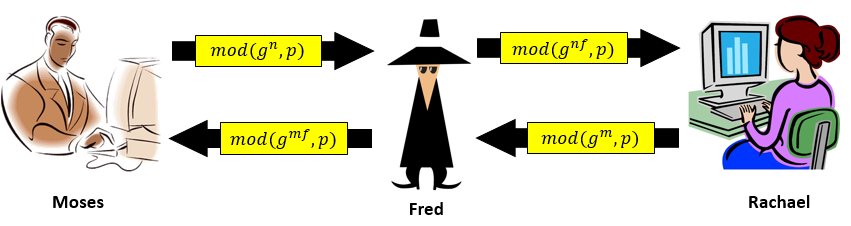
\includegraphics[width=4in]
	         {images/DHKE_2.png}}
	  \caption{\label{fig:DH:DHKE_2} Man in the Middle Attack during Moses and Rachael's Key Exchange }
\end{figure}

Fred establishes a secret key $\bmod ( g^nf, p)$ with Moses and another secret key $\bmod ( g^mf, p)$ with Rachael.  DHKE is vulnerable to this type of Man in the Middle (MiM) attack since Moses cannot verify that Rachael was the originator of the message, and vice-versa.  Two possible solutions to the MiM attack are RSA encryption and elliptic curve cryptography. RSA encryption (see Chapter 5.2.1) allows for a digital signature to be sent within the message. This digital signature serves two purposes: first, it authenticates the origin of the sender and second, it ensures the integrity of the message. If you recall from Chapter 5.2.1, a message is encrypted using the private key and is decrypted using a public key (asymmetric cryptography). In the next section, we will examin the second of these alternatives. 

\section{Elliptic Curve Cryptography}\label{sec:ECC:2}


Elliptic Curve Cryptography (ECC) is one approach to the public key sharing dilemma that offers a smaller security level-to-key lenth ratio (see table below for the relationship  of security and key lengths).  The strength of a cryptography security level is measured in bits (80, 128, 192, 256, etc.), and each security bit represents the number of computational steps necessary to find a solution.  Referencing the table below, we can see that ECC with a 160 bit Finite Field has a similar security level to RSA and Diffie Hellman with $2^{1024}$ bit moduli. To give you an idea of security level strength, "in 2002 it took $10^4$ computers (mainly PCs) running 24 hours a day for 549 days" to solve an EC with a 109 bit Finite Field. 
\begin{figure} [H]
	   \center{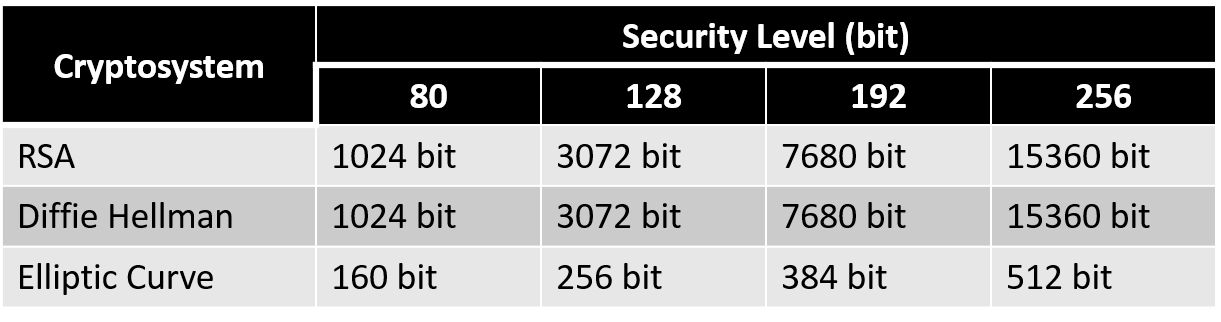
\includegraphics[width=5in]
	         {images/DHKE_9.png}}
	  \caption{\label{fig:DH:DHKE_9} Key bit lengths of Cryptosystems for different security levels }
\end{figure}
The elliptic curve protocol starts from a known point on the elliptic curve called the $generator$.  This point generates the next point which generates the point after that, and the point after that, and so on.  When using ECC, the public key is the point on the elliptic curve, and the private key is the number of iterations or "hops" the generator must make to arrive at the public key point.  In order to use ECC we need to restrict ourselves to Finite Fields (FF) also known as Galois Fields (GF).

\subsection{Elliptic Curves}
The  ECs that we are interested in have a certain geometrical shape E: $y^2 = x^3 + ax + b (\bmod P)$.  See Figure~\ref{fig:DH:DHKE_5} below for a geometrical representation.  
\begin{figure}[H]
	   \center{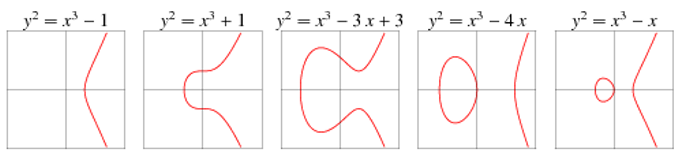
\includegraphics[width=2.5in]
	         {images/DHKE_5.png}}
	  \caption{\label{fig:DH:DHKE_5}   E: $ y^2$ = $x^3+ax+b (\bmod P)$ }
\end{figure}
Furthermore, the EC equation must also satasify the following: $4a^3 + 27b^2 \neq 0$. If $(4a^3)+(27b^2) = 0$ then your elliptic curves have singularities or a self intersection.  See graphs in Figure~\ref{fig:DH:DHKE_10} for a geometrical representation.
\begin{figure}[H]
	   \center{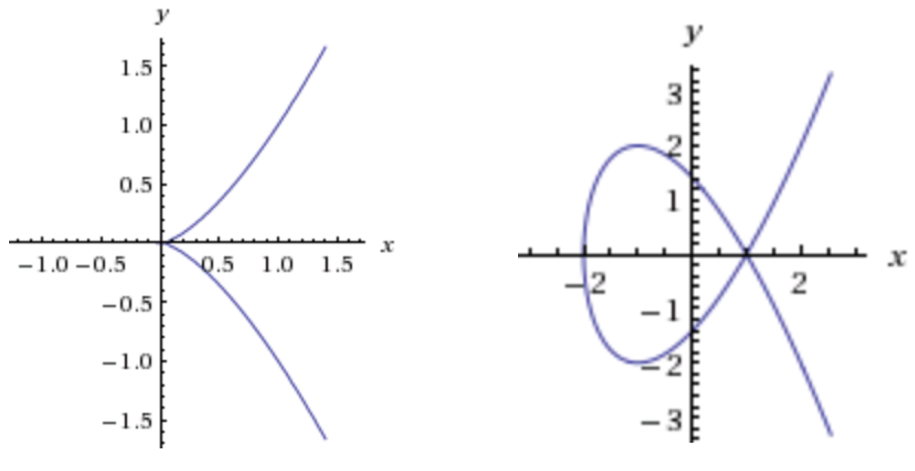
\includegraphics[width=3in]
	         {images/DHKE_10.png}}
	  \caption{\label{fig:DH:DHKE_10} E: $ y^2$ = $x^3$ and E: $ y^2$ = $x^3+ax+b (\bmod P)$ }
\end{figure}

\subsection{Elliptic Curve Groups}
Given the right type of EC we can use the shape of the EC to conduct specific mathematical operations. A group operation, within the parameters of the EC, is sometimes referred to as addition and is given by two points on the EC, $P_1$, $P_2$ $\in$ E then $P_1 + P_2$ = $P_3$ .  The elements of the group are the points on the elliptic curve.  See below for the EC Group Laws.

\begin{enumerate}[1.]
\item \textbf{Identity}: the point at infinity, we'll label this as "0"; 
\item \textbf{Inverse}: given a point $P$, the inverse is the point symmetric about the x-axis;
\item \textbf{closure}: if $P_1$ and $P_2$ are points on the elliptic curve the $P_1 + P_2$ is also a point on the curve;
\item \textbf{associativity}:$(P_1 + P_2) + P_3 = P_1 + (P_2 + P_3)$;
\end{enumerate}


Geometrically if the two points are different then $P_1 + P_2$ is given by drawing a line from point $P_1$ to point $P_2$ and continue the line until it intersects the elliptic curve then reflecting that point about the $x$-axis.  See figure Figure~\ref{fig:DH:DHKE_6} below for a geometrical representation.
\begin{figure}[H]
	   \center{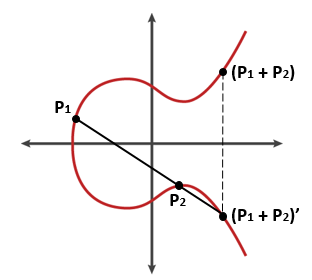
\includegraphics[width=2.5in]
	         {images/DHKE_6.png}}
	  \caption{\label{fig:DH:DHKE_6} }
\end{figure}
Geometrically if the two points are the same then a tangent line to the point is drawn and the resulting operation is then reflected about the x-axis.  This is often referred to as point doubling. See Figure~\ref{fig:DH:DHKE_7} below for a geometrical representation.
\begin{figure}[H]
	   \center{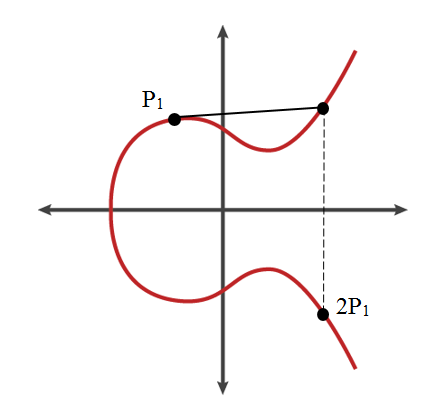
\includegraphics[width=2.5in]
	         {images/DHKE_7.png}}
	  \caption{\label{fig:DH:DHKE_7} }
\end{figure}
**Note, $P_3$ is the Public Key, while the number of hops, $d$, to get to $P_3$ is the Private Key.  In addition, the points on the EC form an abelian group.**

\begin{corollary}
Given E: $y^2 = x^3 + ax + b (\bmod P)$, $P_1 = (x_1, y_1)$, $P_2 = (x_2, y_2)$, and $P_3 = (x_3, y_3)$. Find $P_3$, where $ P_3 =  P_1 + P_2$
\end{corollary}
\begin{enumerate}[(1)] 
	\item The slope $m =(y_2 - y_1)$ $\cdot$ $(x_2- x_1)^{-1}$ $\bmod P$, for $P_1$ $\neq$ $P_2$ \\
		\text{ \qquad \: \:} or $m =(3x^2_1 + a)$ $\cdot$ $(2y_1)^{-1}$ $\bmod P$, for $P_1 = P_2$ 
	\item $x_3 = m^2 - x_1 - x_2 (\bmod P)$ \\
		$y_3 = m(x_1 - x_3) - y_1 (\bmod P)$
	\item For $P^{-1}, m = \infty$ and $P = (x, -y)$ \\
		and $\infty + P = P$, for all $P$
\end {enumerate} 

\begin{eg} Given E: $y^2 = x^3 + 2x + 2 (\bmod17)$, $P_1 = (5,1)$, $P_2 = (5,1)$, and $P_3 = (x_3, y_3)$
	Find $P_3$, where $P_3 = P_1 + P_2$
		\begin{align*}
		\textrm{(1) The slope~} m
		 &= ( (3 \cdot 5^2) + 2) \cdot (2 \cdot 1)^{-1} \bmod 17\\
	          &= (77) \cdot (2)^{-1} \bmod 17\\
                     &\equiv (9) \cdot (9) \bmod 17\\
                     &\equiv 81 \bmod 17\\
                    &\equiv 13
		\end{align*}
		\begin{align*}
		\textrm{(2)~}x_3
		 &= ( (13^2 - 5 - 5  (\bmod 17)) \text{\qquad \qquad \qquad \quad \: \: }\\
	          &= 159(\bmod 17)\\
                     &\equiv 6
		\end{align*}
			\begin{align*}
		\textrm{(3)~}y_3
		 &= ( (13(5 - 6) - 1(\bmod 17)) \text{\qquad \qquad \qquad \quad }\\
	          &= -14(\bmod 17)\\
                     &\equiv 3
		\end{align*}
Thus, $P_3 = (6,3) = 2P$
\end{eg}
\begin {exer}
Using Example 10, find the following: $3P, 4P, 5P, ..., 20P.$  Recall: $3P = 2P + P;  4P = 3P +P;$ etc.  What do you notice about $18P,  19P,$ and $20P?$
\end{exer}
\begin{eg}
Using Example 10 and Exercise 11, let us reconstruct the Diffie Hellman Key Exchange, but this time we'll use the strength of ECC.  Follow along with Figure~\ref{fig:DH:DHKE_8} below.
\end{eg}
\begin{exer}
Using Example 10 and Exercise 11, what is the shared key exchange if Moses chooses $n = 9$ and Rachael chooses $m = 3$?
\end{exer}
\begin{figure}[H]
	   \center{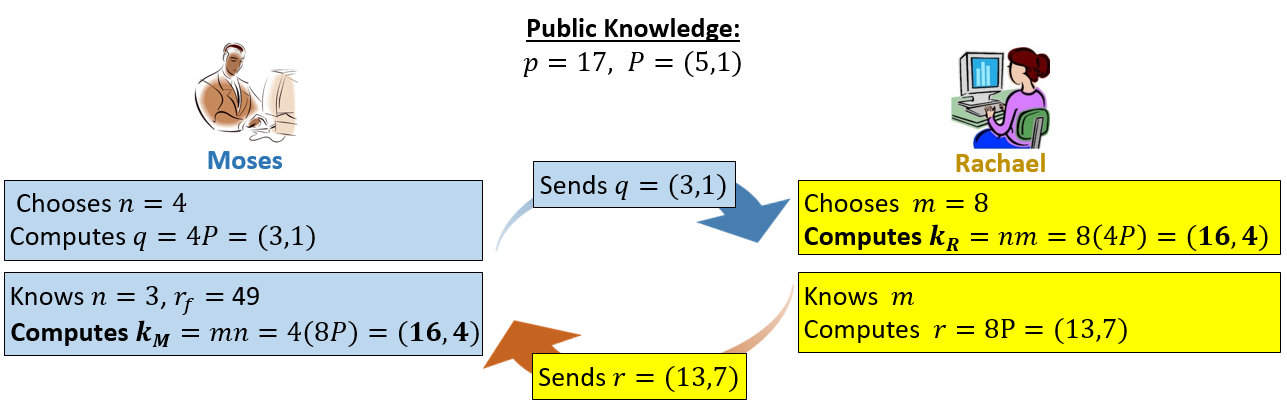
\includegraphics[width=5in]
	         {images/DHKE_8.png}}
	  \caption{\label{fig:DH:DHKE_8} Elliptic Curve Key Exchange between Moses and Rachael }
\end{figure}


\subsection{Galois Field} 
As a review, there are three types of algebraic structures: groups, rings, and fields (see Figure~\ref{fig:DH:DHKE_3}); each structure building from the previous structure.  Each structure is defined as a set of elements where: the given operation is closed, has the identity element, has the inverse element, and is associative.
\begin{figure}[H]
	   \center{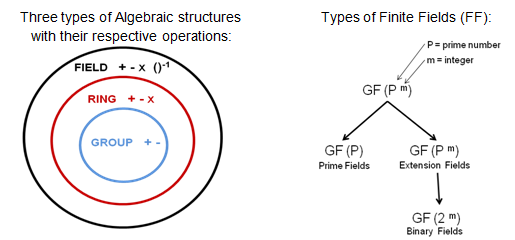
\includegraphics[width=3.5in]
	         {images/DHKE_3.png}}
	  \caption{\label{fig:DH:DHKE_3} Algebraic structures and types of FFs }
\end{figure}
Elliptic curves in $\mathbb{R}$ are not used in practice, because it is impossible for computers to compute decimal fractions exactly.  Instead of $\mathbb{R}$, finite fields are used (finite fields are also called Galois Fields (GF)).  These are preferred, because operations can be computed exactly using integer arithmetic. FFs only exist if they have $P^m$ elements, $GF(P^m)$. So, there is a FF with 27 elements $GF(27) = GF(3^3)$, there is a $FF$ with 256 elements $GF(256) = GF(2^8)$, etc.  In EC we are interested in Binary Fields (BFs), FFs of order $2^m$, with $m ≥ 1$.  Operations in the BF are defined in terms of an irreducible polynomial with degree $m$, this polynomial is also referred to as the reduction polynomial.  This means that the binary polynomial cannot be factored as a product of binary polynomials of degree less than $m$.  As a rule there a $2^m$ elements in $GF(2^m)$, below is an example of the elements in $GF(2^3)$.  
\newline \newline
\begin{eg} Below are the 8 elements of $GF(2^3)$:
\begin{align*}
0, \quad 1, \quad X, \quad X +1, \quad X^2, \quad X^2+1, \quad X^2 + X, \quad X^2 + X + 1
 \end{align*}
\end{eg}
\begin{rem} Given the polynomials $a,b \in  GF(P) = (0,1,2,...,P-1)$ then 
\begin{align*} 		
		a + b &\equiv c (\bmod P)\\
		a - b &\equiv d (\bmod P)\\
		a \cdot b &\equiv e (\bmod P) \quad \text{ ,the multiplicative group does not include 0}\\
		a^{-1} &\equiv b, \mathrm{~if~} a * b (\bmod P) = 1
\end{align*}
\end{rem}	
\begin{eg} Given $GF(2^4)$, then adding two polynomials is as follows:
\begin{align*}
	f(x) &= X^3 + X^2 + X + 1\\
	g(x) &= X^2  + 1\\
           f(x) + g(x) &= X^3  + X
\end{align*}
 \text{Notice that the addition of the coefficient $X^2$ and the constant 1 = 0 in GF($2^4$)}
\end{eg}

\begin{eg} Given $GF(2^8)$, then subtracting two polynomials is as follows:
\begin{align*}	
	f(x) &= X^8 +         X^6 +          X^3 + X^2 + 1\\
	g(x) &=        X^7 + X^6 + X^5 +          X^2\\
 f(x) + g(x) &= X^8 + X^7 +        X^5  + X^3  +         1
\end{align*}
\text{Notice that the binary field has only two coefficients (0,1) so subtraction and}\\
 \text{addition are the same.}
\end{eg}

\begin{eg} Given $GF(2^4)$ and the reduction polynomial $X^4 + X + 1$, then multiplying two polynomials is as follows:
\begin{align*}	
	f(x) &=  X^2 + X + 1\\
	g(x) &= X^3 + 1\\
 f(x) \cdot g(x) &= X^5 + X^4 + X^3 + X^2 + X + 1 (\bmod X^4 + X + 1)\\ 
	       &= - X^3 - X \text{ , is the remainder (see below for explanation) }
\end{align*}
\begin{center}
\begin{tabular}{rrcrcrcrcrcr}
        &  $x$  &  $+$  &      $1$         \\ \cline{2-12}
 \multicolumn{1}{r|}{$x^4 + x + 1$}
        &  $x^5$  &  $+$  &  $x^4$  &  $+$  & $ x^3$  &  $+$  &  $x^2$  &  $+$  & $ x$  &  $+$  &  $1$  \\
        & $x^5$   &  $+$  &       	&          &      	  &          &  $x^2$   & $+$  &  $x$     \\ \cline{2-12}
        &         &       &         $x^4$  & $+$   &  $ x^3$  &   $+$  &             &         &         &          &  $1$  \\
        &         &       &         $x^4$  &  $+$  &             &           &              &         &  $x$   & $+$  &  $1$   \\ \cline{4-12}
        &         &       &                    &          &   $x^3$ &    $-$  &              &         &  $x$    
\end{tabular}
\end{center}
\end{eg}
We proved the following in Exercise~\ref{exercise:modular:71}.

\begin{prop}{BezoutsIdentity}(\emph{Bezout's Identity})~~ let $x$ and $t$ be two-non-zero integers, and let $d$ be their GCD, then there exists integers $p$ and $a$ such that\\
 \hspace*{\parindent} $px + at = d$
\end{prop}

\begin{corollary}
Using Bezout's Identity we can conclude that if $p$ and $a$ are coprime then we have\\
\hspace*{\parindent} $px + at = 1$ \\
reducing $\bmod p$ yields $at = 1 \bmod p$ .  So $t$ is the multiplicative inverse of\\
 $a$ $\bmod n$.
\end{corollary}

\begin{eg} Given $GF(2^8)$ and the reduction polynomial $X^8 + X^4 + X^3 + X +1$, and $a$ = $X^6 + X^4 + X + 1$ then finding the multiplicative inverse of $a$ is as follows:  $a^{-1}$ = $b$, if $a$ $\cdot$ $b$ $(\bmod p)$ = $1$ .  To find $a^{-1}$ use the Extended Euclidian Algorithm.
\\
	$p =  X^8 + X^4 + X^3 + X +1$\\ 
	$a = X^6 + X^4 + X + 1$\\
\\Using the quotients and remainders found below, we can find the multiplicative inverse of $a$ using the following steps \\(new $t$ = old $t - $quotient $\cdot$ $t$):
\begin{enumerate}
\item $t = 0$
\item new $ t = 1$ 
\item new $t = 0 - 1\cdot(x^2 + 1)$
\item  new $t = 1 - (x^4 + x^2)\cdot(x^2 + 1)$
\item new $t = (x^2 + 1) - (x+1)\cdot(x^6 + x^2 + 1)$
\item Stop here and simplify, since the subsequent remainder is 0.
\item new $t = (x^2 + 1) - (x+1)\cdot(x^6 + x^2 + 1)$ = $x^7 + x^6 + x^3 + x$
\end{enumerate}
Thus, $a^{-1}$ = $x^7 + x^6 + x^3 + x$\\
\begin{center}
\begin{tabular}{rrcrcrcrcrcrcr}
        &  $x^2$  &  $+$  &      $1$         \\ \cline{2-14}
 \multicolumn{1}{r|}{$x^6 + x^4 + x + 1$}
        &  $x^8$  &  $+$  &    &      &  $x^4$  &  $+$  & $ x^3$  &  $+$  &   &   & $ x$  &  $+$  &  $1$  \\
        & $x^8$   &  $+$  &    $x^6$      &    $+$         &      &     &  $x^3$  &  $+$  & $x^2$        \\ \cline{2-14}
        &         &              &$x^6$ &$+$ &  $x^4$  & $+$   &              &          & $ x^2$  &   $+$  & $x$   &  $+$  & $1$       \\
        &         &              &$x^6$ &$+$ &  $x^4$  & $+$   &              &          &   &    & $x$   &  $+$  & $1$   \\ \cline{4-14}
        &         &               &          &      &             &           &       &     & $x^2$ 
\end{tabular}
\end{center}

\begin{center}.

\begin{tabular}{rrcrcrcrcrcrcr}
        &  $x^4$  &  $+$  &      $x^2$      \\ \cline{2-8}
 \multicolumn{1}{r|}{$x^2$}
        &  $x^6$  &  $+$  &    $x^4$  &  $+$   & $ x$  &  $+$  &  $ 1$  \\
        & $x^6$     \\ \cline{2-8}
        &              &           &     $x^4$   & $+$  & $x$   &  $+$   & $1$   \\ 
        &              &           &     $x^4$    \\ \cline{4-8}  
        &              &           &                  &          &  $ x$  &  $+$  &  $ 1$  \\
\end{tabular}
\end{center}

\begin{center}
\begin{tabular}{rrcrcrcrcrcr}
        &  $x$  &  $+$  &      $1$      \\ \cline{2-6}
 \multicolumn{1}{r|}{$x + 1$}
        &  $x^2$  \\
        & $x^2$   &  $+$  &    $x$  \\ \cline{2-6}
        &             &          &    $x$   \\
        &             &          &    $x$  & $+$ & $1$ \\ \cline{4-6}
        &             &          &           &        &  $1$
\end{tabular}
\end{center}

\begin{center}
\begin{tabular}{rrcrcrcrcrcr}
        &  $x$  &  $+$  &      $1$      \\ \cline{2-4}
 \multicolumn{1}{r|}{$1$}
        &  $x$      &   $+$ &    $1$  \\
        & $x$     \\ \cline{2-4}
        &             &          &    $1$   \\
        &             &          &    $1$ \\ \cline{3-4}
        &             &          &    $0$
\end{tabular}
\end{center}

\end{eg}

\begin{exer}
What are the binary elements of GF($2^4$)?
\end{exer}
\begin{exer}
Given GF($2^{12}$), then adding $f(X)$+ $g(X)$ = ?
        \\ $f(X)$ = $X^{10} + X^8 + X^5 + X + 1$
        \\ $g(X)$ = $X^{10} + 1$
\end{exer}
\begin{exer}
Given GF($2^4$), then adding $f(X)$ + $g(X)$ = ?
        \\ $f(X)$ = $X^{2} + X $
        \\ $g(X)$ = $X^{3} + 1$
\end{exer}
\begin{exer}
Given GF($2^5$), then subtracting $f(X)$ + $g(X)$ = ?
        \\ $f(X)$ = $X^{4} + X^2 + 1 $
        \\ $g(X)$ = $X^{3} + 1$
\end{exer}
\begin{exer}
Given GF($2^7$), then subtracting $f(X)$ + $g(X)$ = ?
        \\ $f(X)$ = $X^{6} + X^4 + X $
        \\ $g(X)$ = $X^{3} + 1$
\end{exer}
\begin{exer}
Given GF($2^5$) and the reduction polynomial $X^5 + X + 1$ , then multiplying two polynomials, $f(X)$ $\cdot$ $g(X)$ = ?
        \\ $f(X)$ = $X^{3} + X + 1 $
        \\ $g(X)$ = $X^{4} + X$
\end{exer}
\begin{exer}
Given GF($2^5$) and the reduction polynomial $X^5 + X + 1$ , then multiplying two polynomials, $f(X)$ $\cdot$ $g(X)$ = ?
        \\ $f(X)$ = $X^{4} + X^3 + 1 $
        \\ $g(X)$ = $X^{4} + X^2 + X + 1$
\end{exer}
\begin{exer}
Given GF($2^{160}$) and the reduction polynomial $X^{160} + X + 1$ , then multiplying two polynomials, $f(X)$ $\cdot$ $g(X)$ = ?
        \\ $f(X)$ = $X^{120} + X^{100} + 1 $
        \\ $g(X)$ = $X^{80} + X^{70} + X^{60}$
\end{exer}

\subsection{Elliptic Curve Integrated Encryption System} 
If Moses and Rachael would like to communicate a message using ECC, then they could use an agreed upon code table and elliptic curve.  Each character of the encrypted message would correspond to a point on the elliptic curve. Consider an elliptic curve whose equation is $y^2 = x^3 + 2x + 9$, see Figure~\ref{fig:DH:DHKE_11} below.

\begin{figure}[H]
	   \center{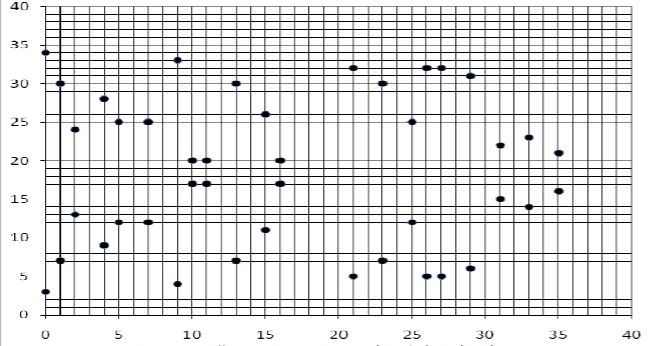
\includegraphics[width=2in]
	         {images/DHKE_11.png}}
	  \caption{\label{fig:DH:DHKE_11} Elliptic Curve, $y^2 = x^3 + 2x + 9$ }
\end{figure}

If we restrict ourselves to the Finite Field, $FF(37)$, so ($y^2 = x^3 + 2x + 9$)$\bmod37$.  Then the points on the elliptic curve are as followed:
($\infty, (5, 25), (1, 30), (21, 32), (7, 25), \newline(25, 12), (4, 28), (0, 34), (16, 17), (15, 26), (27, 32), (9, 4), (2, 24), (26, 5), (33, 14),(11, 17), (31, 22), (13, 30), \newline(35, 21), (23, 7), (10, 17), (29, 6), (29, 31), (10, 20), (23, 30), (35, 16), (13, 7), (31, 15), (11, 20), (33, 23),\newline (26, 32), (2, 13), (9, 33), (27, 5), (15, 11), (16, 20), (0, 3), (4, 9), (25, 25), (7, 12), (21, 5), (1, 7), (5, 12)$)

\newpage 

\subsection{References and Suggested Reading} 
\begin{enumerate}[(1)]

\item
Azad, Saiful, and Pathan, Al-Sakib Khan. "Elliptic Curve Cryptography" in Practical Cryptography, CRC Press, January 2015.

\item 
Bidgoli, Hossein. "Diffie-Hellman Key Exchange" in $Handbook of Information Security: Information Warfare, Social, Legal, and International Issues and Security Foundations, Volume 2$, John Wiley and Sons, January 2006.

\item 
Christensen, Chris. (2015, November 14). $Key Exchanges$. Retrieved from http://www.nku.edu/~christensen/092mat483%20DH%20key%20exchange.pdf.

\item
Franco, Pedro. "Elliptic Curve Cryptography" in $Understanding Bitcoin: Cryptography, Engineering and Economics$, John Wiley and Sons, February 2015.

\item 
Kumar, Suneetha, Chandrasekhar. (2012, January). $Encryption of Data Using Elliptic Curve Over Finite Fields$. Retrieved from https://arxiv.org/ftp/arxiv/papers/1202/1202.1895.pdf.

\item 
Mandal, Surajit, Manna, Nilotpal, and Saha, Arijit. "Diffie-Hellman Key Exchange" in $Information Theory, Coding and Cryptography$, Pearson India, May 2013.





\end{enumerate}